\chapter{AWS Deployment}
\label{Chapter::itAWSDeployment}
\index{AWS Deployment}
\index{Chapter!itAWSDeployment}

\begin{flushleft}
\small{\textit{-- Tamara Gonzalez Ibarra, Michelle Elias Flores, Sydney Winstead}}
\end{flushleft}

\section{AWS Deployment Process}

To deploy our Dockerized website to AWS, we followed the steps outlined in Chapter~3, extending them with our own configuration and automation through a shell script. This section documents our full deployment workflow and provides the exact commands used, formatted with the \texttt{minted} package for clarity.

\subsection{Step 1: Install and Verify AWS CLI}

We first ensured that the AWS Command Line Interface (CLI) was installed and functioning properly on our machines. The CLI is required to authenticate, manage ECR repositories, and create App Runner services directly from the terminal.

\begin{minted}[fontsize=\small,breaklines]{bash}
# Verify that AWS CLI v2 is installed
aws --version
\end{minted}

If the command returned a version number such as \texttt{aws-cli/2.x.x}, we confirmed that AWS CLI was correctly installed.

\subsection{Step 2: Configure AWS SSO Credentials}

Next, we configured AWS Single Sign-On (SSO) to securely access our AWS account without using long-lived access keys. We initialized SSO configuration and created a profile named \texttt{docker-5}.

\begin{minted}[fontsize=\small,breaklines]{bash}
aws configure sso
# SSO session name: my-sso
# SSO start URL: https://d-90662881a4.awsapps.com/start
# SSO region: us-east-1
# Account: 846863293370
# Role: AdministratorAccess
# Default region: us-east-2
# Output format: json
# Profile name: docker-5
\end{minted}

After configuration, we authenticated using SSO:

\begin{minted}[fontsize=\small,breaklines]{bash}
aws sso login --profile docker-5
\end{minted}

This opened a browser window for login verification and returned a success message once authenticated.

\subsection{Step 3: Confirm AWS Credentials}

To ensure that our SSO credentials were valid and linked to the correct AWS account, we verified our caller identity.

\begin{minted}[fontsize=\small,breaklines]{bash}
aws sts get-caller-identity --profile docker-5
\end{minted}

This command returned the account ID, user ARN, and confirmed that our authentication was working correctly.

\subsection{Step 4: Set Environment Variables}

Before deploying, we set environment variables that define our AWS region, repository name, image tag, container port, and application name. These variables were later referenced by our deployment script.

\begin{minted}[fontsize=\small,breaklines]{bash}
export AWS_REGION="us-east-2"
export PROFILE="docker-5"
export ECR_REPO="my-app-repo"
export IMAGE_TAG="latest"
export CONTAINER_PORT=8080
export APP_NAME="my-apprunner-app"
export APP_ROLE_NAME="AppRunnerECRRole"
\end{minted}

\subsection{Step 5: Make the Deployment Script Executable}

We navigated to our project folder \texttt{color-buttons-app} and ensured that the deployment script had executable permissions.

\begin{minted}[fontsize=\small,breaklines]{bash}
cd Documents/color-buttons-app
chmod +x deploy.sh
\end{minted}

\subsection{Step 6: Deploy the Application to AWS}

Finally, we executed our \texttt{deploy.sh} script, which automated the following tasks:

\begin{enumerate}
    \item Creating or reusing an Amazon Elastic Container Registry (ECR) repository.
    \item Authenticating Docker to ECR using a short-lived token.
    \item Building, tagging, and pushing the Docker image to ECR.
    \item Creating or validating an IAM role for App Runner service access.
    \item Deploying the application to AWS App Runner.
    \item Continuously checking the service status until it became \texttt{RUNNING}.
\end{enumerate}

\begin{minted}[fontsize=\small,breaklines]{bash}
./deploy.sh
\end{minted}

The final output confirmed the public URL of our running service:

\begin{quote}
App Runner Service is running at: \url{https://8e4hdgaubu.us-east-2.awsapprunner.com/}
\end{quote}

\subsection{Step 7: Post-Deployment Verification}

After deployment, we tested the provided URL in a browser to ensure that the application loaded successfully and both buttons (blue and red) changed the background color as expected. This confirmed that our Docker image was correctly built, pushed, and deployed on AWS infrastructure.

\subsection{Step 8: Maintenance and Troubleshooting}

To verify future deployments or troubleshoot access, we used the following AWS CLI commands:

\begin{minted}[fontsize=\small,breaklines]{bash}
# List ECR repositories
aws ecr describe-repositories --region us-east-2 --profile docker-5

# Check App Runner service status
aws apprunner list-services --region us-east-2 --profile docker-5

# View service details
aws apprunner describe-service \
    --service-arn <SERVICE_ARN> \
    --region us-east-2 --profile docker-5
\end{minted}

These commands allowed us to monitor the health of our service and ensure that our web application remained accessible after deployment.

\subsection{UML Class Diagram Design}

\begin{figure}[h!]
    \centering
    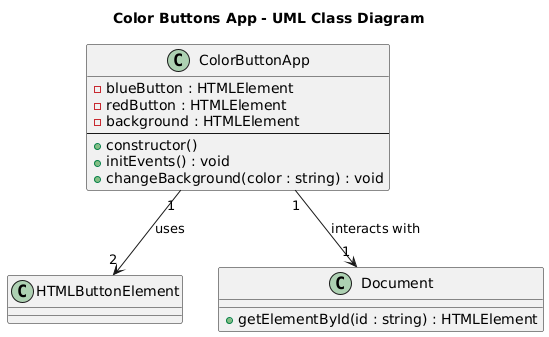
\includegraphics[width=0.8\textwidth]{png/ClassDiagram_Colorbutton.png}
    \caption{Class Diagram for updated class-based java script design}
    \label{fig:umlclassdiagram}
\end{figure}
